\documentclass[conference]{IEEEtran}
\IEEEoverridecommandlockouts
% The preceding line is only needed to identify funding in the first footnote. If that is unneeded, please comment it out.
\usepackage{cite}
\usepackage{amsmath,amssymb,amsfonts}
\usepackage{algorithmic}
\usepackage{graphicx}
\usepackage{textcomp}
\usepackage{xcolor}
\usepackage{multirow}
\usepackage{subcaption}
% \usepackage{caption}
\usepackage[font=footnotesize]{caption}        % controls main caption size
\usepackage{subcaption}
\captionsetup[sub]{font=scriptsize}   % make subcaptions smaller
\usepackage{balance} 

\usepackage{hyperref}
\def\BibTeX{{\rm B\kern-.05em{\sc i\kern-.025em b}\kern-.08em
    T\kern-.1667em\lower.7ex\hbox{E}\kern-.125emX}}

\newenvironment{promptsection}{
  \par\smallskip
  \noindent
  \ttfamily\small
  \setlength{\parindent}{0pt}
  \setlength{\parskip}{0.5em}
}{
  \par\smallskip
  \rmfamily\normalsize
}

\begin{document}

\title{%Profitable Soccer Betting Strategies With Machine Learning and Large Language Models\\
%
%Integrating LLM Sentiment Analysis with Traditional ML Models for Predictive Soccer Betting\\
Integrating LLM Sentiment Analysis into Machine Learning for Soccer Betting\\
}

\author{
\IEEEauthorblockN{
Samuel SAMUEL\textsuperscript{1}\IEEEauthorrefmark{*},
Donghao HUANG\textsuperscript{1,2}\IEEEauthorrefmark{*},
James TAN Yong Hong\textsuperscript{1},
Zhaoxia WANG\textsuperscript{1}
}
\IEEEauthorblockA{\textsuperscript{1}School of Computing and Information Systems, Singapore Management University, Singapore}
\IEEEauthorblockA{\textsuperscript{2}Research and Development, Mastercard, Arlington, VA, USA}
\IEEEauthorblockA{
samuelsamuelgunawan@gmail.com;
dh.huang.2023@smu.edu.sg; james.tan.2021@scis.smu.edu.sg; zxwang@smu.edu.sg
}
\thanks{*Equal contribution.}
}
% samuel1.2021@scis.smu.edu.sg; 
\maketitle

\begin{abstract}
Traditional sports betting models have primarily relied on quantitative statistics, often overlooking the predictive power of qualitative insights such as sentiment from match commentaries. This paper presents a novel hybrid framework that integrates sentiment features generated by advanced Large Language Models (LLMs)—specifically DeepSeek-R1, GPT-4o mini, GPT-4.1, and Qwen2.5-Plus—into conventional machine learning models to enhance soccer betting prediction.
Using a zero-shot prompting approach, we extract sentiment ratings from post-match commentaries and incorporate them as features into logistic regression, SVC, random forest, and XGBoost models under both accuracy- and F1-tuned configurations. Evaluated on nine seasons of English Premier League data (2015–16 to 2023–24), the integrated models demonstrate substantial improvements in betting profitability.
Notably, F1-tuned models consistently outperform their accuracy-tuned counterparts, with the Random Forest model enhanced by GPT-4.1 sentiment features achieving a 279.48\% return, and the XGBoost baseline reaching 247.97\%. The F1-tuned logistic regression model with DeepSeek-R1 sentiment features yielded a 174.01\% return, significantly surpassing traditional approaches.
Our comprehensive evaluation across model architectures and tuning strategies reveals two key findings: (1) F1 optimization is better aligned with profitable sports betting than accuracy optimization, and (2) LLM-derived sentiment features provide varying benefits depending on the underlying algorithm and tuning method. These results underscore the importance of both optimization strategy and qualitative data integration in sports analytics, demonstrating that pre-trained LLMs can effectively capture latent factors often missed by traditional statistical methods, all without requiring additional model training.
\end{abstract}


\begin{IEEEkeywords}
Sports Betting, Machine Learning, Sentiment Analysis, Large Language Models
\end{IEEEkeywords}

\section{Introduction}
Predictive modeling has long been an area of interest for both researchers and industry practitioners, offering a rich testbed for applications such as stock market prediction, which considers both quantitative data and qualitative factors~\cite{wang2023learning,wang2018stock}.
%
%Predictive modeling in complex environments represents a significant challenge in applied data mining research. 
Sports betting markets offer an ideal domain for such predictive modeling research due to their combination of quantitative data, qualitative factors, and clear financial outcomes that enable rigorous performance evaluation. These markets constitute a substantial financial sector characterized by continuous data generation from diverse sources including statistical metrics, performance indicators, and public sentiment-creating rich opportunities for innovative machine learning applications \cite{galekwa2024systematic}.

The integration of machine learning in sports betting has traditionally focused on quantitative statistical features, while qualitative factors such as sentiment from match commentaries have been largely unexplored. This creates a significant research gap as qualitative assessments often contain valuable predictive information that statistical measures alone cannot capture. Addressing this gap requires methodologies that can effectively transform unstructured textual data into usable quantitative features within traditional prediction frameworks.

Our research addresses this challenge through a comprehensive integration methodology with three key components. First, we develop a specialized zero-shot prompting framework that extracts standardized team sentiment scores from unstructured match commentaries, transforming qualitative assessments into quantitative features. Second, we implement a feature engineering approach that combines these sentiment scores with traditional statistical metrics, creating a multi-modal representation that captures both performance patterns and sentiment factors. Third, we establish a systematic evaluation framework that examines the interaction between different Large Language Models (LLMs) architectures and machine learning models.

The focus of the study is on soccer betting, particularly the 1X2 (win, draw, or away) bet in the English Premier League (EPL). The EPL is one of the most popular leagues in the world, and the 1X2 betting market is the most popular form of soccer betting, providing an ideal testbed for our methodological approach.

The main contributions of this research are as follows:
\begin{itemize}
\item The paper proposes a novel method that incorporates sentiment features from advanced LLMs (DeepSeek-R1, GPT-4o mini, GPT-4.1 and Qwen2.5-Plus) into traditional machine learning models, enhancing predictive performance in sports betting.
\item This work presents
the first comprehensive study on integrating the latest LLMs
capabilities in sentiment analysis to traditional machine learning
models for sports betting.
\item  The proposed method is empirically validated on English Premier League betting, where LLM-based sentiment features improve the performance of traditional models, as demonstrated by a significant increase in returns.
\item The study provides new insights into how sentiment analysis from LLMs interacts with and enhances the performance of conventional machine learning algorithms in the context of sports betting.
\item This work represents a significant step forward in the application of LLMs for sentiment analysis in sports betting, demonstrating the potential for qualitative factors captured by LLMs to outperform traditional approaches.
% \item Upon acceptance, we will release our codebase with all the parameters, to
% support future research in sports betting.
\item The complete codebase and all associated parameters are available in a public GitHub repository\footnote{Public Repository URL: \url{https://github.com/SSSamueLDS/Integrating-LLM-Sentiment-Analysis-into-Machine-Learning-for-Soccer-Betting}} to support future research in sports betting.
\end{itemize}

This paper is organized as follows: Section II reviews related works on machine learning in sports betting and LLMs in sentiment analysis. Section III describes the datasets used and their preprocessing. Section IV details our methodological framework, including the zero-shot prompting approach and experimental design. Section V presents our experimental results and discussion, highlighting the performance variations across different model architectures. Finally, Section VI concludes with implications for sports betting research and potential future directions.

%The focus of the study is on soccer betting, particularly the 1X2 (win, draw, or away) bet in the English Premier League (EPL). The EPL is one of the most popular leagues in the world, and the 1X2 betting market is the most popular form of soccer betting, providing an ideal testbed for our methodological approach.

%Upon acceptance, we will release our codebase and LLM sentiment analysis results along with all the parameters, to support future research in sports betting.


\section{Related Works}
This section explores related works on machine learning in sports betting, as well as the usage of LLMs in sentiment analysis of textual data.

\noindent\textbf{Machine Learning for Soccer Betting}
There are many different algorithms used for machine learning in sports betting, such as support vector machines (SVC), random forests, multi-layer perceptron (MLP), and deep neural networks. Machine learning models have significantly improved prediction accuracy and enhanced risk management. Some pertinent challenges of machine learning in sports betting include the high risk of overfitting due to the limited number of events, picking relevant features that reflect the complexities of the sport, and the immense amount of computational resources needed to train a model with many features \cite{galekwa2024systematic}.

One of the more recent models used for sports betting is the XGBoost model. A study by Terawong et al. (2024) has shown that using XGBoost can enhance betting performance. It was found that real-time learning from dynamic market simulations leads to more profitable wagering decisions. This shows the suitability of the XGBoost algorithm in capturing complex non-linear relationships in the complex, fast-changing environment of sport betting \cite{terawong2024xgboost}.

There are also techniques in feature engineering in sports betting which are used to reduce the number of features while still making sure that the data is meaningful. One approach used is to take the difference between the home and away teams' statistics, so that two features can be reduced into one \cite{walsh2024machine}. Since the feature is a relative figure between teams and not an absolute figure, it is less prone to shift over time as the characteristics of a sporting league may change over time \cite{dutta2017identifying}.

Another technique used in feature selection is to convert sentiment data into numerical features so that it can be trained together with other numerical data in ML models. This has been used in predicting the movement in stock prices, where news sentiment numerical features were trained together with technical indicator data on traditional ML models. Incorporating sentiment data was shown to improve the accuracy of stock price trend prediction \cite{attanasio2019combining}. The transferability from stock price prediction to soccer betting is high as both are financial markets which involve large amounts of data.

\noindent\textbf{LLMs for Text Sentiment Analysis}
Recent months have witnessed intense competition among companies releasing Large Language Models (LLMs), including OpenAI (GPT), DeepSeek, and Alibaba (Qwen). OpenAI's GPT-4o, released in May 2024, demonstrated superior text understanding performance \cite{islam2024gpt4o}, while their April 2025 GPT-4.1 introduced a 1 million token context window with 21\% improvement on coding benchmarks and 10.5\% enhancement in instruction-following tasks \cite{openai2025gpt41}. DeepSeek-R1, trained using large-scale reinforcement learning, showed superior reasoning ability compared to GPT-4o \cite{deepseek2025r1}. Alibaba's Qwen2.5-Plus achieved comparable performance to GPT-4o while being more economical \cite{qwen2025technical}.

The utilization of LLMs for sentiment analysis—including applications in Chinese language—will be one of the key directions for future research~\cite{wang2025review}. Huang and Wang (2025) evaluated GPT-4o and DeepSeek-R1 on fine-grained sentiment analysis using Amazon Reviews data. In zero-shot settings, GPT-4o achieved 74.32\% accuracy while DeepSeek-R1 reached 78.31\% accuracy on 1-5 star rating predictions \cite{huang2025explainable}, demonstrating that current LLMs can achieve nuanced textual understanding without labeled examples.

% There have been many Large Language Models (LLMs) released in recent months, with intense competition between companies such as OpenAI (GPT), DeepSeek, and Alibaba (Qwen). GPT-4o was released by OpenAI in May 2024, showing superior performance in understanding texts \cite{islam2024gpt4o}. Thereafter, DeepSeek released DeepSeek-R1, a model that is trained using large-scale reinforcement learning, which demonstrated superior reasoning ability when compared to GPT-4o \cite{deepseek2025r1}. At around the same time as DeepSeek, Alibaba released its Qwen2.5 models, of which its Qwen2.5-Plus model performed comparably to GPT-4o while being more economical \cite{qwen2025technical}.

% After the release of the LLMs, a study by Huang and Wang (2025) explored the performance of LLMs on fine-grained sentiment analysis. GPT-4o and DeepSeek-R1 were used to predict the ratings of reviews from 1 to 5 stars on the Amazon Reviews data set, which is widely used for the study of sentiment analysis. With 0 shots (no labelled examples in the prompt), GPT-4o achieved an accuracy of 74.32\% while DeepSeek-R1 achieved an accuracy of 78.31\% \cite{huang2025explainable}. This shows that the most current LLMs can get a nuanced understanding of textual data without prior specific examples for reference.

%\noindent\textbf{Emotion AI with Commonsense for Interpretable Affective Computing}
A growing body of work fuses affect modeling with commonsense knowledge to achieve
both stronger performance and interpretability. Concept-level sentiment analysis
(SenticNet) shifts from word-level polarity to \emph{concept}-level appraisal, linking
semantics, affect, and commonsense relations \cite{cambria2013statistical,cambria2023seven}.
The Hourglass of Emotions provides a psychologically motivated structure for mapping
text to affective dimensions and primary emotions \cite{susanto2020hourglass}. Recent
neurosymbolic approaches integrate knowledge graphs, conceptual primitives, and
reasoning for explainable sentiment understanding \cite{li2024primenet,cambria2024understanding}.
% This line of work emphasizes \emph{interpretable cues} (e.g., “clinical finishing,”
% “wasteful in possession,” “organized pressing”) that connect events and appraisals to
% affect. 
% Our LLM-based sentiment feature is designed to capture these concept-level
% signals in zero-shot fashion; in Section~\ref{sec:interpretability}, we show how
% captured rationales enhance transparency and how concept-aware baselines compare.

\section{Dataset}
\noindent\textbf{Data Sources and Collection Methods}
Firstly, EPL soccer match statistics from the 2015-16 to 2023-24 seasons (9 years) were obtained from 
API-Football\footnote{\url{https://www.api-football.com}}, a paid API 
service. Statistics include total shots by team, shots on 
goal, fouls, ball possession (\%), and yellow/red cards.

Secondly, betting odds for the 2023-24 season 
were obtained from Football-Data.co.uk\footnote{\url{http://www.football-data.co.uk/englandm.php}}. Specifically, average 1X2 pre-match betting odds from BetFair were 
obtained for the EPL matches. 1X2 refers to betting 
on either a home win, draw, or away win.

Thirdly, post-match commentaries for each soccer match from the 2015-16 to the 2023-24 seasons 
(9 years) were obtained from BBC Sports\footnote{\url{https://www.bbc.com/sport}}. 
%The relevant URLs to each match commentary were obtained through Google searches. Searches were automated by using Google Custom Search API\footnote{\url{https://developers.google.com/custom-search/v1/overview}} to get the search results and DeepSeek-V3 API\footnote{\url{https://api-docs.deepseek.com/}} to choose the relevant URLs from the search results. Manual checks were performed to ensure the correct URL was obtained for each match. 
Web scraping using the Python Selenium 
library\footnote{\url{https://github.com/SeleniumHQ/Selenium}} was then performed using the obtained URLs to get the article text.

\noindent\textbf{Training and Evaluation Data Partitioning}
The entire dataset comprises 9 seasons (2015-16 to 2023-24 seasons) except for the betting odds data which is only used on the betting simulation (2023-24 season only). Data partitioning: 2015–19 for feature selection/hyperparameter tuning; 2015–22 for training; 2022–23 for testing; 2023–24 for betting simulation.
%The data is split as follows:
%\begin{enumerate}
    %\item Feature selection and hyperparameter tuning set (4 seasons, 2015-16 to 2018-19 seasons)
    %\item Training set (7 seasons, 2015-16 to 2021-22 seasons)
    %\item Testing set (1 season, 2022-23 season)
%    \item Final training set (8 seasons, 2015-16 to 2022-23 seasons)
    %\item Betting simulation set (1 season, 2023-24 season)
%\end{enumerate}


\section{Proposed Methodological Framework}

\noindent\textbf{Overview of the proposed methodology}
% Figure~\ref{fig_wide} depicts our methodology as a flowchart.
Figure~\ref{fig_wide} presents a comprehensive overview of our integrated methodology framework. The flowchart illustrates the systematic approach that bridges traditional sports analytics with modern LLM capabilities. The framework is organized into four interconnected modules that work synergistically to enhance betting performance. 

The Data Collection module (a) combines quantitative soccer match statistics with qualitative BBC match commentaries, providing the foundation for both statistical and sentiment-based features. The LLM Sentiment Analysis module (b) represents our novel contribution, where we leverage four state-of-the-art LLMs (DeepSeek-R1, GPT-4o mini, GPT-4.1, Qwen2.5-Plus) to extract nuanced sentiment scores from textual match commentaries. This module transforms unstructured text into standardized numerical features using a 5-point sentiment scale, with the final sentiment feature computed as the relative difference between the home and away team sentiments. The Machine Learning Models \& Learning Pipeline module (c) implements a rigorous process that includes correlation-based feature removal, sequential forward selection for optimal feature subsets, grid search hyperparameter optimization, and systematic evaluation across four different model architectures. Finally, the Betting Simulation module (d) validates our approach through a realistic financial simulation using the Kelly criterion for optimal bet sizing\cite{kelly1956new}, ensuring that our methodology translates into practical betting strategies with positive expected returns.

\begin{figure}
\centering
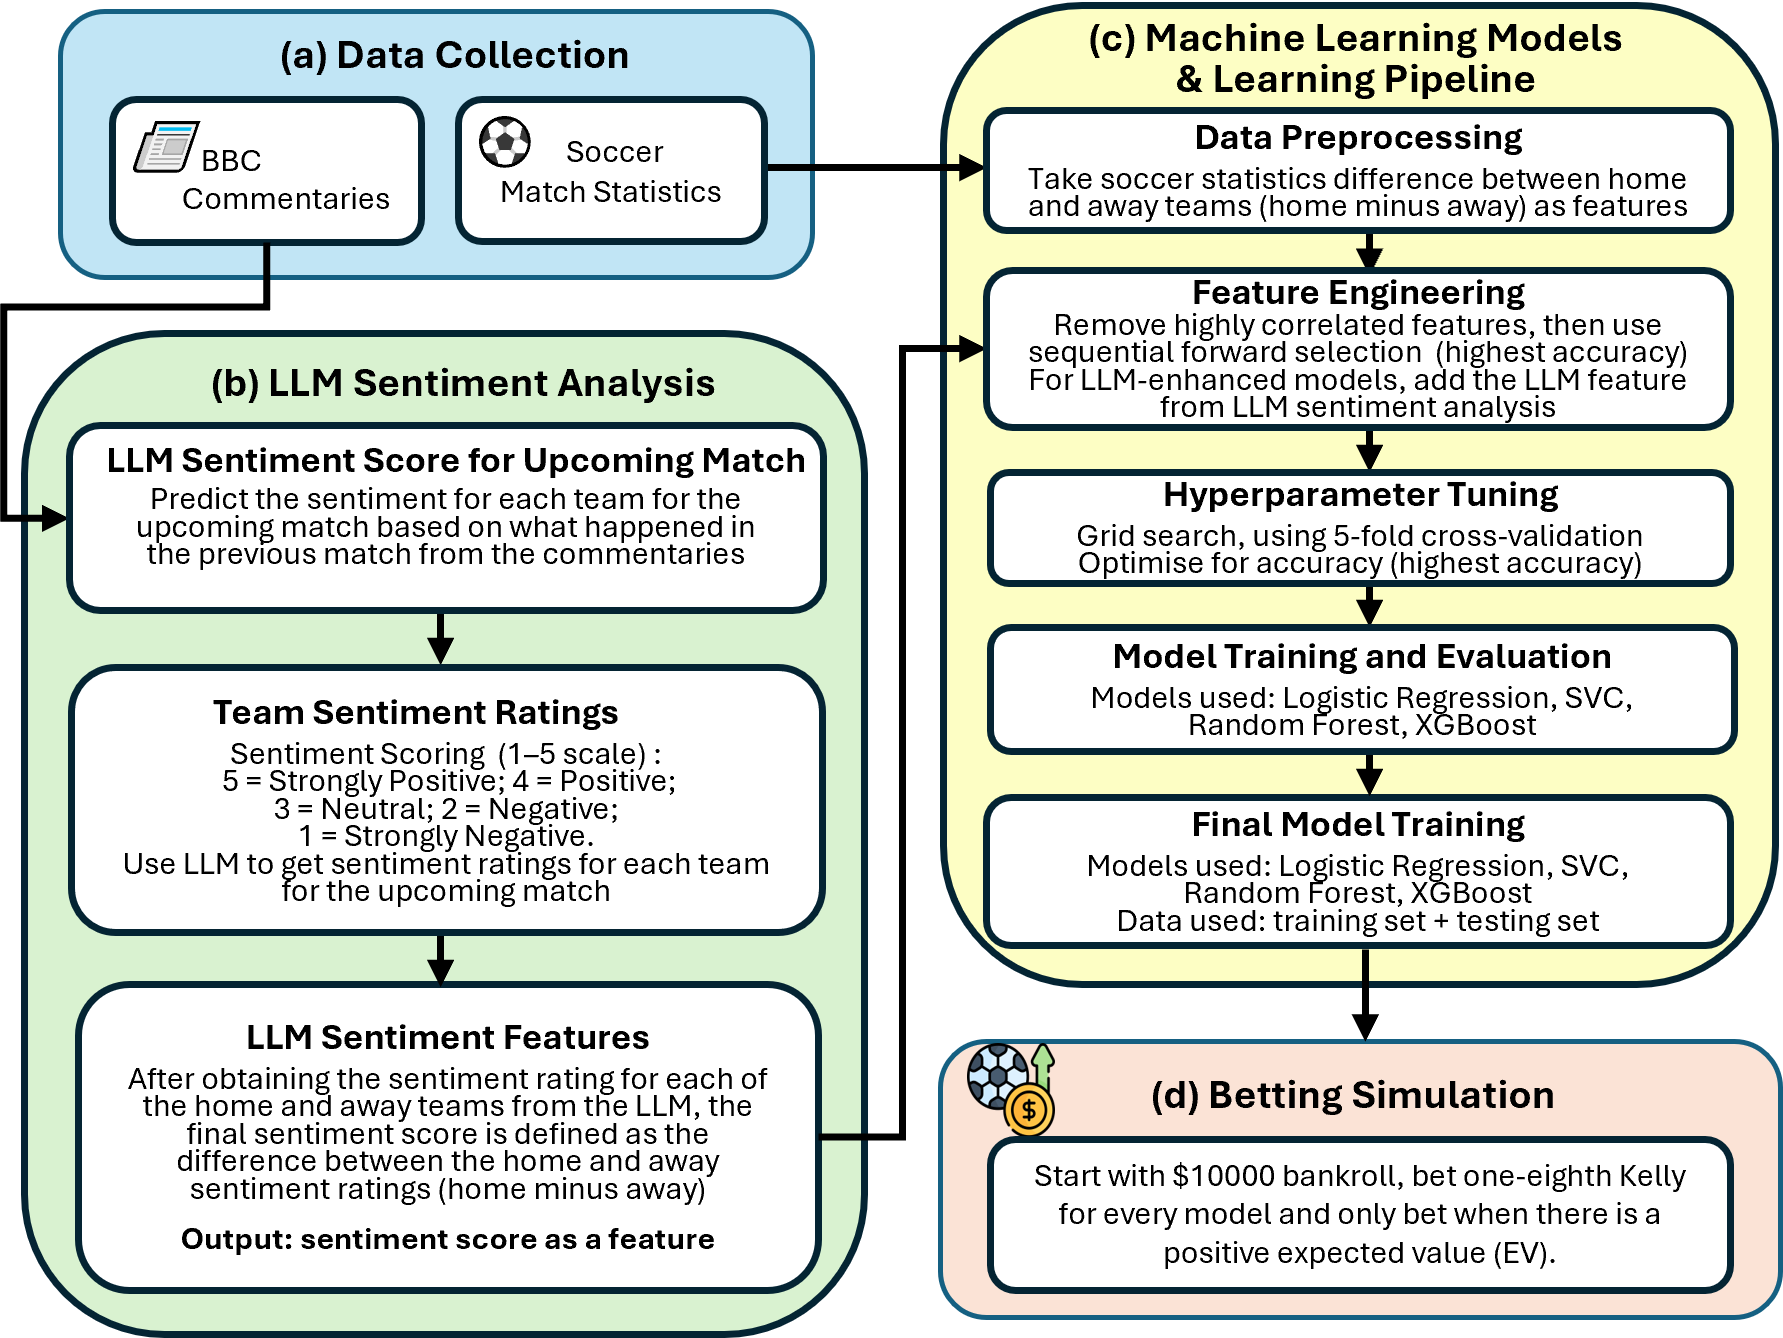
\includegraphics[width=\columnwidth]{images/metholodogy flowchart_v5.1.png}
\caption{Overview of the LLM-Enhanced Sports Betting Prediction Framework. The flowchart depicts a four-stage pipeline: 
(a) \textbf{Data Collection}—soccer match statistics are retrieved from API-Football, and post-match commentaries are scraped from BBC Sport; 
(b) \textbf{LLM Sentiment Analysis}—Large Language Models (DeepSeek-R1, GPT-4o mini, GPT-4.1, Qwen2.5-Plus) generate team-level sentiment ratings on a 1–5 scale based on prior match commentaries. A sentiment feature is computed as the difference between the home and away team ratings; 
(c) \textbf{Machine Learning Pipeline}—statistical and sentiment features are combined, followed by preprocessing (decorrelation, feature selection), hyperparameter tuning via grid search and 5-fold cross-validation, and training with four models: Logistic Regression, SVC, Random Forest, and XGBoost; 
(d) \textbf{Betting Simulation}—a simulated bankroll of \$10{,}000 is used with one-eighth Kelly betting\cite{kelly1956new}. Bets are placed only when a positive expected value condition is satisfied.}
\label{fig_wide}
\end{figure}

\noindent\textbf{LLM Sentiment Analysis
%Data Preprocessing
}
To obtain current sentiment data for each match, the BBC Sport commentary article for the most recent English Premier League (EPL) match played by the home team before the target upcoming match in the current season was retrieved. The same was done for the away team. Subsequently, the online APIs of DeepSeek-R1, GPT-4o Mini, GPT-4.1, and Qwen2.5-Plus were queried using the prompt shown below. Each model was tasked with providing a sentiment rating from 1 to 5 (as illustrated in module (b) of Figure~\ref{fig_wide} for both the home and away teams, based on the commentary of their respective most recent matches. The fields in square brackets were replaced with the relevant team-specific information. These four models were selected for their strong performance and cost-effectiveness.

% To obtain the current sentiment data for each match, the BBC Sports commentary article for the last match the home team played in the EPL in the current season was found. This was also done for the away team. Next, the online APIs of DeepSeek-R1, GPT-4o mini, GPT-4.1, and Qwen2.5-Plus were called with the following prompt below to obtain a sentiment rating of 1 to 5 (as illustrated in module (b) of Figure~\ref{fig_wide}) on both the home and away teams separately based on the commentary for their respective previous matches, with the fields in square brackets replaced by the relevant information. DeepSeek-R1, GPT-4o mini, GPT-4.1, and Qwen2.5-Plus were chosen due to their performance and cost-effectiveness.


\begin{promptsection}
\footnotesize
You are an advanced sentiment analysis assistant. Your task is to 
analyze match commentaries in the English Premier League. The sentiment 
rating on a certain team should be based on a 5-point scale:
Strongly Positive (5), Positive (4), Neutral (3), Negative (2), or 
Strongly Negative (1).

I would like you to predict the sentiment for each team for the 
upcoming match based on what happened in the previous match. For the 
upcoming match on \textcolor{teal}{[match\_date]}, \textcolor{teal}{[home\_team]} is the
home team and \textcolor{teal}{[away\_team]} is the away team. I have found the BBC 
commentaries of both teams' previous matches.

Rate the sentiment of each team on an output on a scale of 1-5. Reply 
in a JSON format with the following keys: home\_team\_sentiment, 
away\_team\_sentiment. Do not reply with anything else.

Below are the articles:

The article for \textcolor{teal}{[home\_team]}'s previous match on 
\textcolor{teal}{[home\_team\_last\_match\_date]}:
\textcolor{teal}{[home\_team\_commentary]}

The article for \textcolor{teal}{[away\_team]}'s previous match on 
\textcolor{teal}{[away\_team\_last\_match\_date]}:
\textcolor{teal}{[away\_team\_commentary]}
\end{promptsection}


After obtaining the sentiment rating for both the home and away teams from each LLM, the difference between the home and away sentiment ratings was obtained (home minus away) for each LLM. This resulted in a separate sentiment data feature for each LLM. These sentiment scores are leveraged by the machine learning models, as shown in Figure~\ref{fig_wide}.

\noindent\textbf{Machine Learning
Models \& Learning Pipeline
%General Experimental Approach
}
%Our general experimental approach consists of 4 steps, with each step using the relevant datasets stated previously:
For machine learning models, our experimental approach consists of four steps as shown in Figure~\ref{fig_wide}, Module (c), each utilizing the relevant datasets mentioned previously:

%\begin{enumerate}

%    \item Data Preprocessing

%    \item Feature Engineering
%    \item Hyperparameter tuning using grid search and 5-fold cross-validation
%    \item Model Training (including initial model training and testing, \&
%    final model training)
    %\item Betting simulation
%\end{enumerate}
\subsubsection{Data Preprocessing}
For each match, compute 5‑match and season‑to‑date averages for home and away, then take home‑minus‑away differences; exclude each team’s first five matches.
%For every EPL match in each season, the average was found for both the home and away team separately for each match statistic (such as shots taken, shots on target, corner kicks, and fouls) for the past five matches and for all past matches in that season. After that, the difference between the home team and away team (home minus away) was obtained for each match statistic. This was to find the short-term and long-term relative performance between the home and away teams before each match occurred, and to also reduce the number of features in the dataset used for training. The first five matches for each team in every season were removed since the statistics for the last five matches in the season could not be found. This was also done so that the models could make a more informed decision.
\subsubsection{Feature Engineering}
The feature engineering process followed a methodology similar to that described in \cite{walsh2024machine}. %Feature selection was conducted in two stages. First, features with a Spearman correlation coefficient greater than 0.7 were grouped, and only the first feature from each group was retained to reduce multicollinearity. Next, sequential forward selection was applied using logistic regression as the learning algorithm. At each step, the feature subset that achieved the highest match outcome prediction accuracy—based on model calibration—was selected as the optimal subset. 
Remove highly correlated features (Spearman > 0.7), then apply sequential forward selection using logistic regression. 
This process resulted in the selection of eight features.
For LLM-enhanced models, a sentiment feature was added separately for each LLM variant, bringing the total number of features to nine.
% The steps were similar to those in Joshi et al (2024). Feature selection was done in two steps. Firstly, highly correlated features with a Spearman coefficient of more than 0.7 were
% grouped together and the first feature in each group was retained. Next, sequential forward selection was done with logistic regression as the learning algorithm. For each step, the feature subset with the highest accuracy in predicting the match outcome is considered the optimal feature subset based on calibration. There were 8 features selected in total. The sentiment data feature was added separately for each of the LLM variants, making a total of 9 features for LLM-enhanced models.
\subsubsection{Hyperparameter tuning} We used grid search with 5-fold cross-validation to optimise our hyperparameters. The objective function used during tuning was accuracy and F1 score. 

\subsubsection{Model Training}


We used four models: logistic regression, support vector classification (SVC), random forest, and XGBoost. All models %except for XGBoost 
are traditional machine learning models. The initial training was performed with the training set (7 seasons, 2015-16 to 2021-22 seasons) and tested with the testing set (1 season, 2022-23 season) to obtain the initial training and testing results. 

\subsubsection{Model Evaluation}
The models were evaluated in accuracy, F1 score, and log loss. Accuracy and F1 score were chosen to reflect the classification ability of the model, while log loss indicates the quality of probability estimates--crucial for actual betting. Accuracy metric can be less reliable when classes are imbalanced especially in sports betting, as it treats all prediction errors equally regardless of class distribution.
F1 score provides a more nuanced evaluation and is particularly valuable in sports betting contexts where the frequency of wins, draws, and losses may vary significantly.
Log loss captures how well
the predicted probabilities align with the actual class labels, a
critical factor in determining optimal bet sizing for profitable
wagering strategies. For a three-class classification problem, the expected log loss from random guessing would be approximately
1.1. A lower log loss indicates that the model’s predictions are
more accurate and well-calibrated. 
\subsubsection{Final Model Training}
The final training, with the model tested on the betting simulation dataset (2023-24 season, 1 season), used the training and testing sets combined (2015-16 to 2022-23 seasons, 8 seasons) for training. The same hyperparameters obtained from initial model training and used on testing was also used for the final model training.

\noindent\textbf{Betting Simulation
}We used the Kelly method \cite{kelly1956new} for bet sizing, which considers the probability of winning to maximise wins and minimize losses. The Kelly criterion for determining the optimal bet size is calculated as:

\begin{equation}
f^* = \frac{p \cdot b - (1-p)}{b}\label{eq1}
\end{equation}

\noindent where:
\begin{itemize}
\item   $f *$ is the fraction of the current bankroll to wager
\item $p$ is the probability of winning
\item $b$ is the odds received on the bet (represents the potential winnings on a wager of 1 unit)
\end{itemize}
Specifically, one-eighth of the usual Kelly bet was used to minimize the risk of ruin \cite{hsieh2015kelly}. Using this method allows more to be bet when the model is more confident of choosing the correct outcome, with the maximum loss limited to 12.5\% of the portfolio. Betting is only done on positive‑EV opportunities. Our betting simulation operates under two assumptions: unlimited bet sizing and perfect market liquidity.
%when the odds given by the bookmaker are better than the odds implied by the model for a betting option. Kelly betting was chosen for the betting simulation because the simulation's approach directly aligns with Kelly principles where bets are only placed when there is a positive expected value (EV). Furthermore, it most accurately reflects the disciplined bankroll management strategies employed by sports bettors in real-world scenarios.


%Our betting simulation operates under three key assumptions. First, we assume unlimited bet sizing with no minimum or maximum betting constraints, allowing the Kelly criterion to determine optimal stake sizes without artificial limitations. Second, we assume perfect market liquidity, meaning all calculated bet amounts can be executed at the quoted odds without market impact or slippage. Third, we assume no additional transaction costs beyond the bookmaker's margin embedded in the odds, as contemporary sportsbooks typically do not impose separate transaction fees, deriving profit exclusively from their built-in odds margins.

We mainly evaluate the quality of the betting models through betting returns in percent. Starting with an initial bankroll of \$10000, betting is done sequentially following chronological match order, excluding the first five matches of each team due to insufficient historical data for reliable prediction. %The model evaluation follows a systematic procedure where predictions are generated for each qualifying match in chronological sequence, betting decisions are executed based on model outputs and corresponding bookmaker odds, bankroll adjustments are calculated following each match outcome, and the process iterates sequentially through all remaining fixtures until season completion. 


%The first 5 matches for every season are not used in the experiments since there is not enough prior data to make an informed decision.

% \subsection{
% Betting Simulation
% }

%\cite{walsh2024machine}. 



\section{Experimental Results and Discussion}

\noindent\textbf{Predictive Accuracy and Probability Calibration Analysis}

Table~\ref{tab:accuracy_calibration_results} presents the testing results, displaying the F1 score, accuracy, and log loss of each model under two different tuning approaches: accuracy-tuned and F1-tuned configurations. 

The results reveal distinct performance patterns between accuracy-tuned and F1-tuned configurations across model architectures when enhanced with LLM-derived sentiment features. All models achieve accuracy between 49.09\% and 53.94\% on the testing dataset, with F1 scores ranging from 40.37\% to 46.91\%. For Logistic Regression, accuracy-tuned models show baseline and Qwen2.5-Plus achieving the highest accuracy at 53.94\%, while F1-tuned configurations demonstrate superior F1 performance with Qwen2.5-Plus reaching 46.91\%. Notably, GPT-4o mini consistently provides the best log loss performance in both tuning approaches (0.9950 for accuracy-tuned, 0.9956 for F1-tuned), indicating superior probability calibration.

SVC models exhibit interesting trade-offs between tuning strategies. While accuracy-tuned baseline achieves 53.64\% accuracy, the F1-tuned variants show more balanced performance metrics. Random Forest demonstrates the most pronounced differences between tuning approaches, with F1-tuned GPT-4o mini achieving the highest F1 score (45.89\%) despite a significant increase in log loss (1.0812), suggesting potential overfitting or calibration issues. XGBoost shows relatively stable performance across both tuning strategies, with F1-tuned GPT-4.1 providing the best balance of metrics (43.66\% F1, 51.21\% accuracy, 1.0259 log loss).

The comparison between tuning strategies reveals that F1-tuned models do not universally outperform accuracy-tuned variants. In many cases, accuracy-tuned models maintain competitive F1 scores while achieving better probability calibration, as evidenced by lower log loss values. This finding is particularly relevant for betting applications, where well-calibrated probabilities are crucial for accurate assessment of betting value and optimal stake sizing. The mixed results suggest that the choice between accuracy and F1 tuning should be informed by the specific requirements of the betting strategy and the relative importance of precision versus recall in the classification task.

Contrary to initial expectations, LLM-enhanced versions do not consistently outperform baseline models across all metrics and tuning strategies. However, the analysis reveals that different LLM variants excel in different aspects: DeepSeek-R1 and GPT-4o mini consistently demonstrate improved probability calibration with lower log loss values, while GPT-4.1 and Qwen2.5-Plus show better performance in specific model-tuning combinations. This heterogeneous performance pattern suggests that the optimal LLM enhancement strategy may be model-dependent and should be selected based on the specific performance priorities of the betting application.

\begin{table*}[htbp]
\caption{Testing performance comparison between the baseline and LLM-infused variations for the 4 different machine learning models. Best performing results for each model category are highlighted in bold.}
\label{tab:accuracy_calibration_results}
\centering
\scriptsize
\renewcommand{\arraystretch}{1.2}
\begin{tabular}{l l c c c c c c}
\hline
\multirow{2}{*}{\textbf{Model}} & \multirow{2}{*}{\textbf{Sub-model}} & \multicolumn{3}{c}{\textbf{Accuracy-Tuned}} & \multicolumn{3}{c}{\textbf{F1-Tuned}} \\
\cline{3-8}
& & \textbf{F1 Score (\%)} & \textbf{Accuracy (\%)} & \textbf{Log Loss} & \textbf{F1 Score (\%)} & \textbf{Accuracy (\%)} & \textbf{Log Loss} \\
\hline
\multirow{5}{*}{Logistic Regression} 
& Baseline & \textbf{46.78} & \textbf{53.94} & 1.0038 & 46.30 & 53.33 & 1.0074 \\
& DeepSeek-R1 & 45.38 & 52.73 & \textbf{0.9980} & 45.11 & 52.12 & 1.0013 \\
& GPT-4o mini & 43.17 & 50.61 & 1.0087 & 45.64 & 52.42 & \textbf{0.9956} \\
& GPT-4.1 & 45.04 & 52.42 & 0.9974 & 46.66 & 53.64 & 0.9991 \\
& Qwen2.5-Plus & 44.81 & 52.12 & 1.0041 & \textbf{46.91} & \textbf{53.94} & 0.9966 \\
\hline
\multirow{5}{*}{SVC}
& Baseline & \textbf{46.20} & \textbf{53.64} & 1.0106 & \textbf{46.20} & \textbf{53.64} & 1.0135 \\
& DeepSeek-R1 & 45.38 & 52.73 & 1.0111 & 45.38 & 52.73 & 1.0111 \\
& GPT-4o mini & 45.17 & 52.12 & \textbf{1.0064} & 45.51 & 51.82 & 1.0213 \\
& GPT-4.1 & 46.02 & 53.03 & 1.0045 & 43.06 & 50.61 & 1.0177 \\
& Qwen2.5-Plus & 45.93 & 53.03 & 1.0098 & 45.93 & 53.03 & \textbf{1.0086} \\
\hline
\multirow{5}{*}{Random Forest}
& Baseline & 40.37 & 50.30 & 1.0151 & 42.29 & 50.61 & \textbf{1.0072} \\
& DeepSeek-R1 & 42.88 & 50.91 & 1.0071 & 42.40 & 49.09 & 1.0173 \\
& GPT-4o mini & \textbf{43.19} & \textbf{51.21} & 1.0121 & \textbf{45.89} & 50.00 & 1.0812 \\
& GPT-4.1 & 41.65 & 50.61 & 1.0100 & 43.25 & 49.39 & 1.0208 \\
& Qwen2.5-Plus & 42.58 & 50.30 & \textbf{1.0045} & 44.13 & \textbf{50.91} & 1.0101 \\
\hline
\multirow{5}{*}{XGBoost}
& Baseline & 42.80 & 50.30 & 1.0347 & 43.65 & 50.30 & \textbf{1.0160} \\
& DeepSeek-R1 & 43.11 & 50.30 & \textbf{1.0183} & 42.16 & 49.09 & 1.0202 \\
& GPT-4o mini & \textbf{43.73} & \textbf{51.21} & 1.0267 & 43.18 & 50.00 & 1.0432 \\
& GPT-4.1 & 43.43 & 50.91 & 1.0343 & \textbf{43.66} & \textbf{51.21} & 1.0259 \\
& Qwen2.5-Plus & 41.87 & 49.39 & 1.0508 & 43.06 & 50.61 & 1.0280 \\
\hline
\end{tabular}
\end{table*}

\noindent\textbf{Profitability Analysis and LLM Enhancement Impact}

Table~\ref{tab:betting_simulation_results} presents the betting simulation results for the baseline and LLM-enhanced variations across the four machine learning models under both accuracy-tuned and F1-tuned configurations. The simulation was conducted on the 2023-24 EPL season with an initial bankroll of \$10,000, encompassing 330 matches after excluding the first five matches for each team from model training and betting simulation.

The results reveal significant variability in how different machine learning architectures and tuning strategies respond to LLM enhancement for betting applications. A striking pattern emerges when comparing tuning strategies: F1-tuned models consistently achieve superior performance compared to their accuracy-tuned counterparts across nearly all configurations. The top-performing results are dominated by F1-tuned models, with Random Forest GPT-4.1 achieving an exceptional 279.48\% return, XGBoost baseline reaching 247.97\%, and Logistic Regression DeepSeek-R1 delivering 174.01\%. This systematic superiority of F1-tuned models suggests that optimizing for balanced precision and recall is fundamentally better aligned with profitable sports betting than traditional accuracy optimization.

The comparison between accuracy-tuned and F1-tuned models demonstrates that tuning strategy profoundly impacts betting profitability, often more than the choice of LLM enhancement itself. This finding has critical implications for sports betting applications, where the optimization objective during model training directly influences real-world financial outcomes. The consistent outperformance of F1-tuned configurations indicates that sports betting prediction benefits from models that maintain balanced performance across all outcome classes rather than maximizing overall accuracy.

%Among accuracy-tuned baseline models, three architectures demonstrated profitability: Logistic Regression (75.12\%), SVC (72.18\%), and XGBoost (8.30\%), while Random Forest incurred substantial losses (-21.01\%). However, F1-tuned configurations dramatically altered this landscape, with Random Forest baseline achieving 113.96\% returns—representing a 135 percentage point improvement over its accuracy-tuned counterpart. Similarly, XGBoost baseline improved from 8.30\% to 247.97\% when F1-tuned, while Logistic Regression and SVC baselines also showed gains (105.22\% and 33.07\% respectively).

The impact of LLM-derived sentiment features varied dramatically across model types and tuning strategies, revealing complex interactions between architecture, optimization objective, and sentiment integration. Logistic Regression models demonstrated exceptional responsiveness to LLM enhancement, particularly in F1-tuned configurations. DeepSeek-R1 achieved the most outstanding performance with 174.01\% returns (F1-tuned) compared to 89.35\% (accuracy-tuned), representing improvements of 68.79 and 14.23 percentage points over their respective baselines. This suggests that DeepSeek-R1's sentiment features are particularly well-suited for Logistic Regression's linear decision boundaries when optimized for balanced precision and recall.

SVC models exhibited contrasting responses between tuning strategies. While accuracy-tuned SVC showed limited benefit from LLM enhancement—with only the baseline achieving meaningful profitability (72.18\%)—F1-tuned configurations demonstrated substantial improvements. GPT-4o mini achieved 89.81\% returns in F1-tuned mode versus 19.12\% in accuracy-tuned mode, indicating that SVC's decision boundaries benefit significantly from F1 optimization when incorporating sentiment features.

Random Forest models displayed the most dramatic transformation patterns, particularly highlighting the critical importance of tuning strategy. While accuracy-tuned Random Forest generally struggled (best performance: Qwen2.5-Plus at 65.54\%), F1-tuned configurations achieved exceptional results. GPT-4.1 delivered extraordinary returns of 279.48\%, representing a 272.16 percentage point improvement over the accuracy-tuned baseline. DeepSeek-R1 also performed exceptionally well with 164.76\% returns in F1-tuned mode compared to 22.03\% in accuracy-tuned mode. This suggests that Random Forest's ensemble methodology thrives when sentiment features are integrated with F1 optimization.

XGBoost models revealed the most complex interaction patterns between tuning strategies and LLM enhancement. While accuracy-tuned XGBoost showed modest baseline performance (8.30\%) with DeepSeek-R1 achieving notable improvements (92.07\%), F1-tuned configurations demonstrated even more dramatic results. The F1-tuned baseline achieved exceptional returns of 247.97\%, representing a 239.67 percentage point improvement over the accuracy-tuned baseline. However, LLM enhancements in F1-tuned XGBoost generally underperformed the baseline, suggesting that the F1-tuned baseline may have reached near-optimal performance for this dataset.

The results reveal highly architecture and tuning-specific patterns for LLM effectiveness. DeepSeek-R1 demonstrated exceptional performance with F1-tuned Logistic Regression (174.01\%) and accuracy-tuned XGBoost (92.07\%), but showed more modest gains with other configurations. GPT-4.1 excelled particularly with F1-tuned Random Forest (279.48\%), while GPT-4o mini showed consistent improvements across multiple model-tuning combinations, making it the most versatile LLM enhancement tested.

%The betting frequency analysis reveals additional insights into model behavior. Both accuracy-tuned and F1-tuned models generally placed similar bet counts (321-328 range), with minimal variation between tuning strategies. The consistency in betting frequency across configurations suggests that the probability threshold effects are relatively stable, with performance differences primarily attributable to improved probability calibration rather than betting volume changes.

These findings demonstrate that the interaction between model architecture, tuning strategy, and LLM enhancement is highly complex and non-linear. The optimal configuration requires systematic evaluation of all three factors simultaneously, as superior performance in one combination does not predict success in others. Most significantly, the results show that F1 tuning can fundamentally transform model profitability, often delivering greater improvements than LLM enhancement alone. This underscores the critical importance of alignment between model optimization objectives and real-world application requirements in sports betting systems.

\begin{table*}[htbp]
\caption{Betting simulation results for the baseline and LLM-enhanced variations for each of the 4 different models (initial bankroll: \$10,000). Best performing results for each model category are highlighted in bold.}
\label{tab:betting_simulation_results}
\centering
\scriptsize
\renewcommand{\arraystretch}{1.2}
\begin{tabular}{l l c c c c c c}
\hline
\multirow{2}{*}{\textbf{Model}} & \multirow{2}{*}{\textbf{Sub-model}} & \multicolumn{3}{c}{\textbf{Accuracy-Tuned}} & \multicolumn{3}{c}{\textbf{F1-Tuned}} \\
\cline{3-8}
& & \textbf{Final Bankroll} & \textbf{Return (\%)} & \textbf{Number of Bets} & \textbf{Final Bankroll} & \textbf{Return (\%)} & \textbf{Number of Bets} \\
\hline
\multirow{5}{*}{Logistic Regression} 
& Baseline & 17511.62 & 75.12 & 327 & 20521.53 & 105.22 & 328 \\
& DeepSeek-R1 & \textbf{18934.66} & \textbf{89.35} & 326 & \textbf{27401.07} & \textbf{174.01} & 327 \\
& GPT-4o mini & 12709.69 & 27.10 & 324 & 21063.95 & 110.64 & 327 \\
& GPT-4.1 & 17952.08 & 79.52 & 325 & 16001.87 & 60.02 & 326 \\
& Qwen2.5-Plus & 14197.88 & 41.98 & 324 & 17503.85 & 75.04 & 327 \\
\hline
\multirow{5}{*}{SVC}
& Baseline & \textbf{17218.18} & \textbf{72.18} & 325 & 13307.05 & 33.07 & 321 \\
& DeepSeek-R1 & 12502.31 & 25.02 & 325 & 12502.31 & 25.02 & 325 \\
& GPT-4o mini & 11912.11 & 19.12 & 328 & \textbf{18980.86} & \textbf{89.81} & 323 \\
& GPT-4.1 & 9062.88 & -9.37 & 324 & 12111.53 & 21.12 & 325 \\
& Qwen2.5-Plus & 15177.75 & 51.78 & 326 & 18117.17 & 81.17 & 324 \\
\hline
\multirow{5}{*}{Random Forest}
& Baseline & 7899.23 & -21.01 & 324 & 21395.57 & 113.96 & 326 \\
& DeepSeek-R1 & 12202.58 & 22.03 & 324 & 26476.16 & 164.76 & 325 \\
& GPT-4o mini & 8401.30 & -15.99 & 321 & 7997.07 & -20.03 & 327 \\
& GPT-4.1 & 10732.30 & 7.32 & 323 & \textbf{37948.34} & \textbf{279.48} & 325 \\
& Qwen2.5-Plus & \textbf{16554.05} & \textbf{65.54} & 324 & 17403.54 & 74.04 & 326 \\
\hline
\multirow{5}{*}{XGBoost}
& Baseline & 10830.16 & 8.30 & 327 & \textbf{34797.11} & \textbf{247.97} & 326 \\
& DeepSeek-R1 & \textbf{19206.61} & \textbf{92.07} & 322 & 13315.21 & 33.15 & 324 \\
& GPT-4o mini & 9444.86 & -5.55 & 326 & 8391.48 & -16.09 & 328 \\
& GPT-4.1 & 10571.70 & 5.72 & 326 & 13005.82 & 30.06 & 323 \\
& Qwen2.5-Plus & 8645.57 & -13.54 & 328 & 12426.54 & 24.27 & 323 \\
\hline
\end{tabular}
\end{table*}

\noindent\textbf{Temporal Patterns and Market Timing Analysis}

Figures~\ref{fig:all_bankroll_evolution} and~\ref{fig:all_bankroll_evolution_f1} detail the temporal evolution of bankroll during the betting simulation for the 2023-24 EPL season across the various machine learning models and their LLM-enhanced variations under both accuracy-tuned and F1-tuned configurations. The simulation encompasses 330 matches instead of the usual 380 matches due to the exclusion of the first five matches for each team from model training and betting simulation.

The bankroll trajectories reveal distinct temporal patterns that provide crucial insights into model performance beyond simple accuracy metrics, with dramatic differences between tuning strategies. Most accuracy-tuned models exhibit a characteristic pattern: an initial decline period (matches 0-100), followed by varying growth phases, with significant volatility throughout the season. However, F1-tuned models demonstrate fundamentally different temporal characteristics, often showing more aggressive growth patterns and higher peak values, confirming the superior profitability outcomes observed in the final results.

\subsubsection{Accuracy-Tuned Model Performance}

For accuracy-tuned Logistic Regression models (Figure~\ref{fig:all_bankroll_evolution}(a)), the LLM-enhanced variants, particularly DeepSeek-R1, demonstrated exceptional ability to capitalize on profitable opportunities throughout the season. DeepSeek-R1 showed dramatic surges starting around match 250, reaching peaks above 30,000 units before settling at the final performance. The baseline model showed more modest and consistent growth, while GPT-4o mini demonstrated volatile performance with significant declines in the latter portion of the season.

SVC models (Figure~\ref{fig:all_bankroll_evolution}(b)) exhibited more modest performance overall, with the baseline achieving the most consistent growth pattern. GPT-4o mini showed strong mid-season performance with peaks around matches 150-200, while other LLM variants demonstrated more volatile patterns with mixed outcomes.

The accuracy-tuned Random Forest results (Figure~\ref{fig:all_bankroll_evolution}(c)) reveal a fundamentally different pattern that explains their poor profitability outcomes. The baseline Random Forest showed consistent decline throughout the season, confirming its poor final performance. However, the LLM-enhanced variants, particularly Qwen2.5-Plus, demonstrated modest improvements with more stable performance through the season's end.

XGBoost models (Figure~\ref{fig:all_bankroll_evolution}(d)) showed the most dramatic contrast between baseline and LLM performance in accuracy-tuned configurations. The DeepSeek-R1 variant demonstrated exceptional growth, reaching peaks above 19,000 units around match 250. This variant showed consistent growth from match 150 onwards with remarkable late-season performance, while other variants showed declining or modest performance.

\subsubsection{F1-Tuned Model Performance}

The F1-tuned configurations (Figure~\ref{fig:all_bankroll_evolution_f1}) reveal dramatically different temporal patterns that explain their superior final performance. F1-tuned Logistic Regression models (Figure~\ref{fig:all_bankroll_evolution_f1}(a)) show even more pronounced growth patterns than their accuracy-tuned counterparts. DeepSeek-R1 achieves exceptional performance with sustained growth throughout the season, while GPT-4o mini also demonstrates strong consistent performance, contrasting sharply with its accuracy-tuned volatility.

F1-tuned SVC models (Figure~\ref{fig:all_bankroll_evolution_f1}(b)) exhibit remarkable transformation from their accuracy-tuned performance. GPT-4o-mini achieves outstanding growth with steady upward trajectory, reaching much higher peak values than any accuracy-tuned SVC variant. The baseline and other LLM variants also show improved stability and growth patterns compared to accuracy-tuned configurations.

The most striking transformation occurs with F1-tuned Random Forest models (Figure~\ref{fig:all_bankroll_evolution_f1}(c)). GPT-4.1 demonstrates extraordinary performance, achieving exceptional growth patterns that culminate in the highest final returns observed across all model configurations (279.48\%). The baseline Random Forest also shows dramatic improvement, transitioning from consistent losses in accuracy-tuned mode to substantial gains. DeepSeek-R1 exhibits strong mid-to-late season performance with sustained growth patterns.

F1-tuned XGBoost models (Figure~\ref{fig:all_bankroll_evolution_f1}(d)) present the most complex temporal patterns. The baseline configuration achieves exceptional performance with dramatic late-season growth, reaching the second-highest final returns (247.97\%). However, most LLM-enhanced variants show more modest performance, suggesting that the F1-tuned baseline may have reached near-optimal calibration for this dataset.

\subsubsection{Comparative Temporal Analysis}

The comparison between accuracy-tuned and F1-tuned temporal patterns reveals several critical insights. First, F1-tuned models generally demonstrate more aggressive growth trajectories and achieve higher peak values, consistent with their superior final profitability. 

Second, the timing of profitable periods varies significantly between tuning strategies, with F1-tuned models often showing sustained growth patterns rather than the volatile swings characteristic of accuracy-tuned models.

% Third, volatility patterns differ markedly between tuning approaches. Accuracy-tuned models frequently exhibit dramatic swings with periods of substantial gains followed by significant retracements, while F1-tuned models tend toward more sustained directional movement. This suggests that F1 optimization produces better probability calibration for betting applications, resulting in more consistent identification of profitable opportunities.

Finally, the analysis demonstrates that LLM enhancement effects vary dramatically between tuning strategies. While certain LLM-model combinations show exceptional performance in accuracy-tuned configurations (e.g., DeepSeek-R1 with Logistic Regression and XGBoost), F1-tuned configurations often achieve superior results with different LLM combinations or even baseline models. This indicates that the interaction between tuning strategy, model architecture, and sentiment features is highly complex and requires empirical evaluation for optimal performance.

The temporal analysis reinforces that F1 tuning fundamentally transforms model behavior in betting applications, often delivering not just better final outcomes but also more favorable risk-adjusted performance through reduced volatility and more consistent growth patterns. This has important implications for practical betting applications where sustained performance and risk management are critical considerations beyond simple profitability metrics.

\begin{figure*}[htbp]
\centering
\subfloat[Logistic Regression\label{fig:logistic_bankroll}]{%
    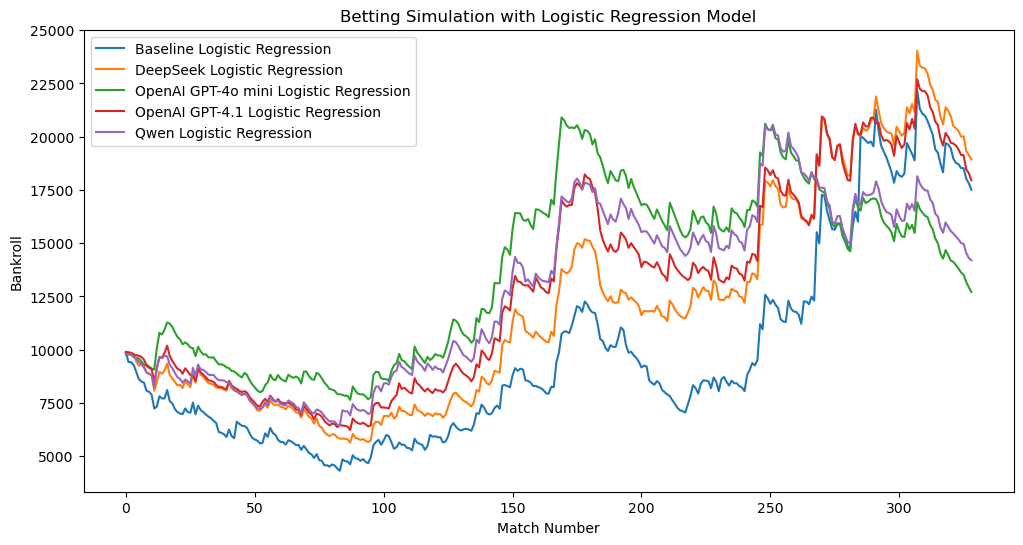
\includegraphics[width=0.48\textwidth]{images/lr_acc_kelly.png}
}
\hfill
\subfloat[SVC\label{fig:svc_bankroll}]{%
    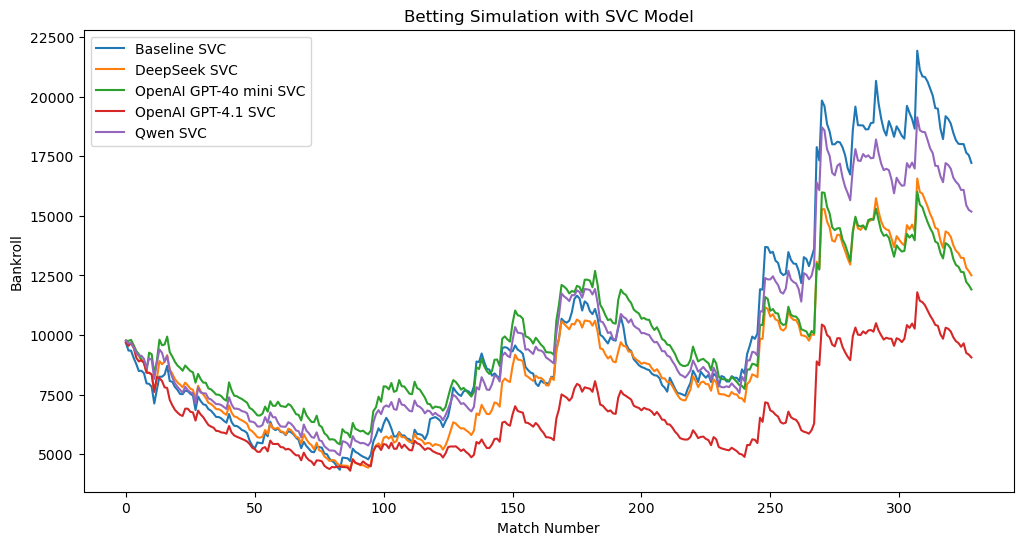
\includegraphics[width=0.48\textwidth]{images/svc_acc_kelly.png}
}

\vspace{0.1cm}

\subfloat[Random Forest\label{fig:random_forest_bankroll}]{%
    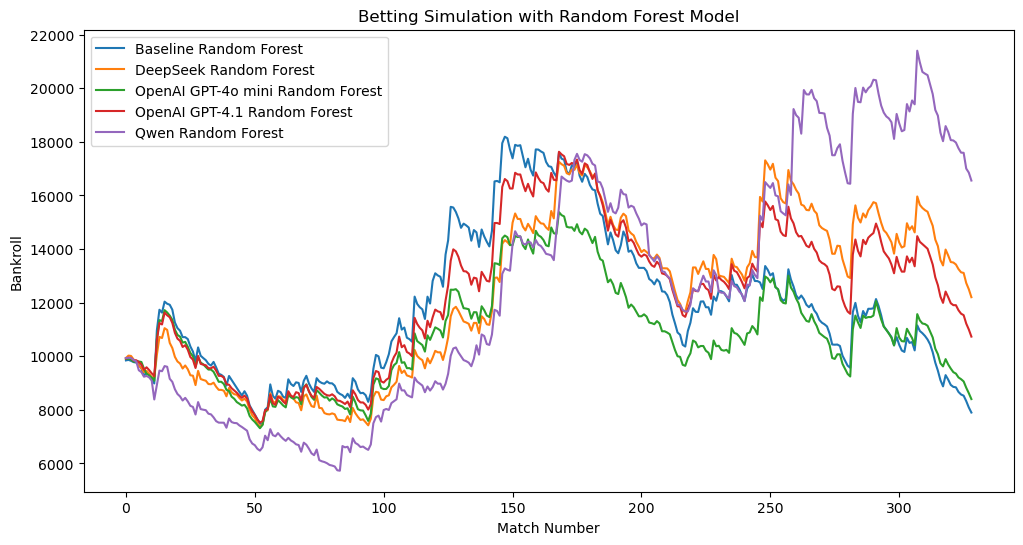
\includegraphics[width=0.48\textwidth]{images/rf_acc_kelly.png}
}
\hfill
\subfloat[XGBoost\label{fig:xgboost_bankroll}]{%
    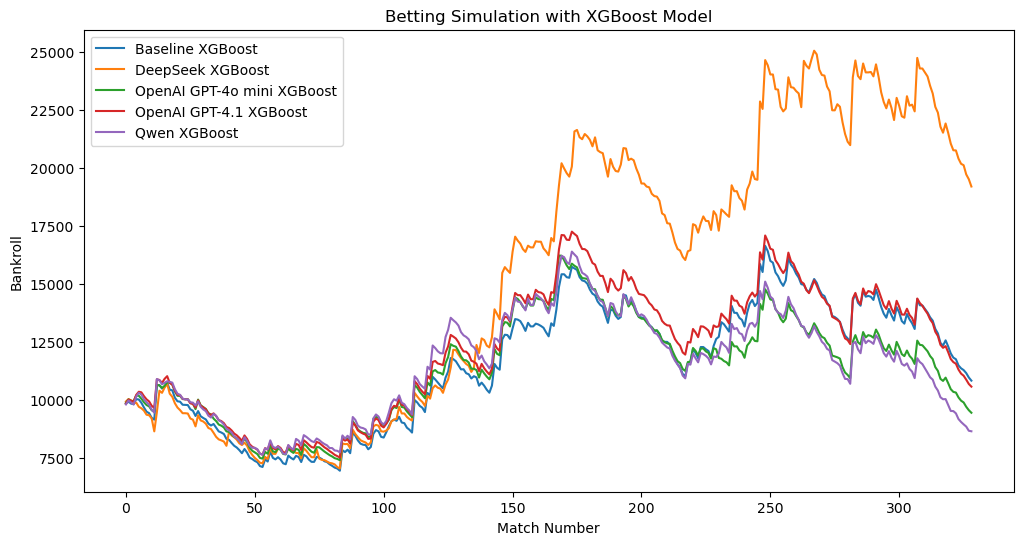
\includegraphics[width=0.48\textwidth]{images/xgboost_acc_kelly.png}
}

\caption{Betting simulation bankroll evolution across matches for the 2023-24 EPL season comparing accuracy-tuned baseline models with their LLM-infused variations across four different machine learning architectures.}
\label{fig:all_bankroll_evolution}
\end{figure*}

\begin{figure*}[htbp]
\centering
\subfloat[Logistic Regression\label{fig:logistic_bankroll_f1}]{%
    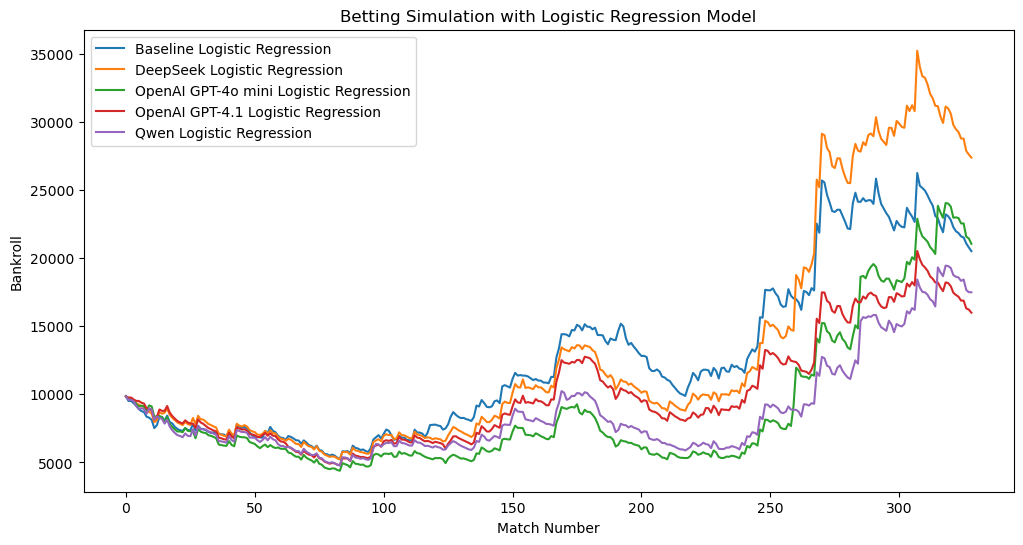
\includegraphics[width=0.48\textwidth]{images/lr_f1.png}
}
\hfill
\subfloat[SVC\label{fig:svc_bankroll_f1}]{%
    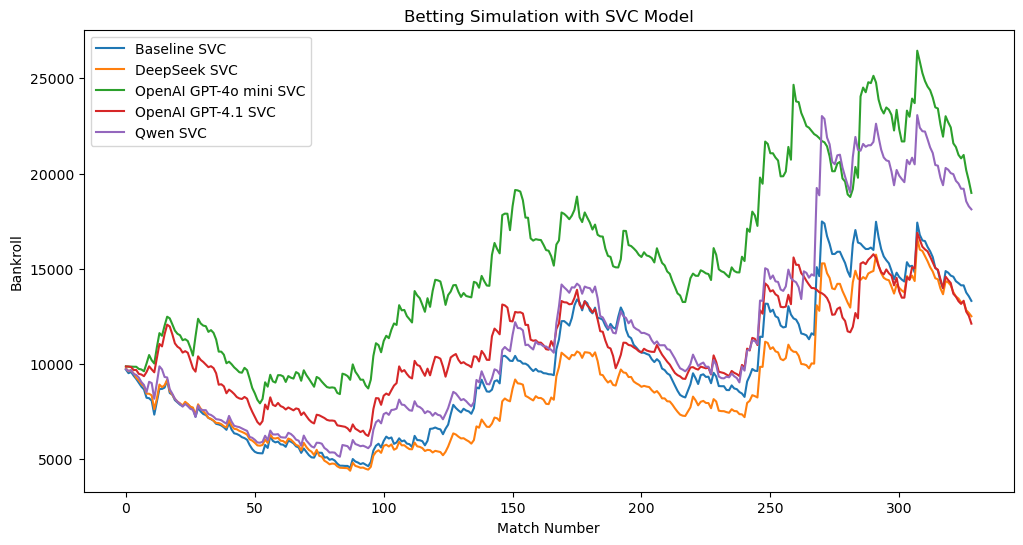
\includegraphics[width=0.48\textwidth]{images/svc_f1.png}
}

\vspace{0.1cm}

\subfloat[Random Forest\label{fig:random_forest_bankroll_f1}]{%
    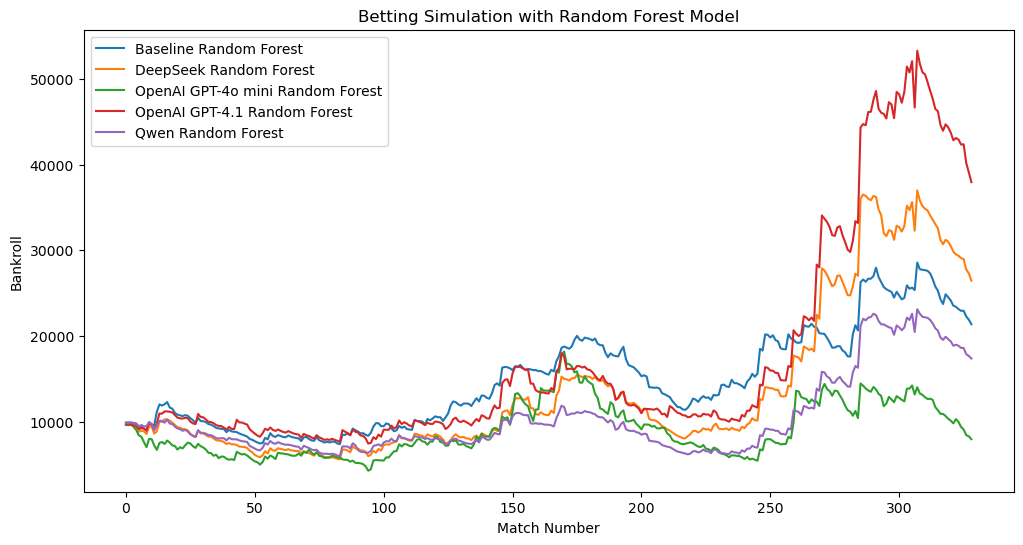
\includegraphics[width=0.48\textwidth]{images/rf_f1.png}
}
\hfill
\subfloat[XGBoost\label{fig:xgboost_bankroll_f1}]{%
    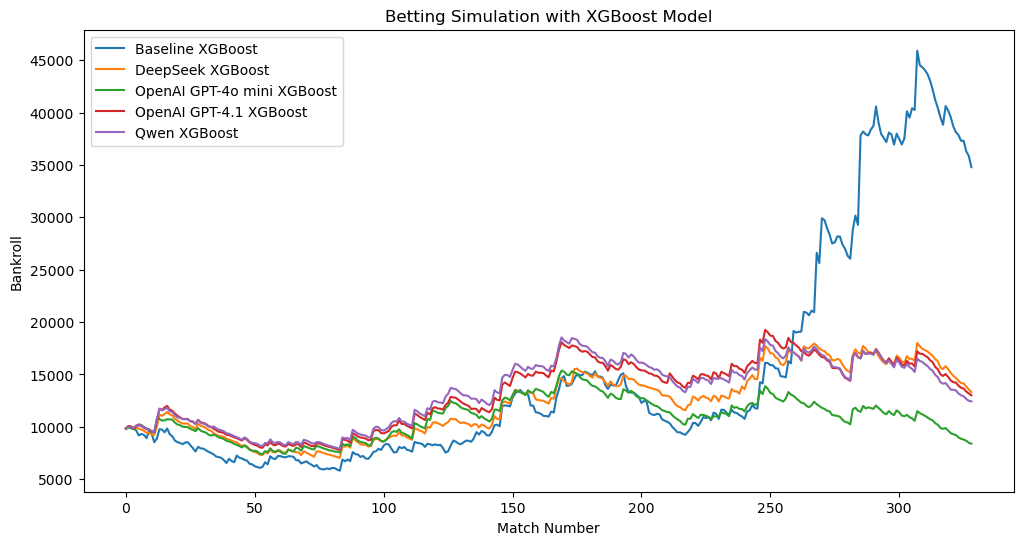
\includegraphics[width=0.48\textwidth]{images/xgboost_f1.png}
}

\caption{Betting simulation bankroll evolution across matches for the 2023-24 EPL season comparing F1-tuned baseline models with their LLM-infused variations across four different machine learning architectures.}
\label{fig:all_bankroll_evolution_f1}
\end{figure*}

\section{Conclusion}
This study demonstrates the substantial practical and financial value of integrating LLM-derived sentiment features into traditional machine learning models for soccer betting prediction. Our comprehensive evaluation across four model architectures, four advanced LLMs, and two tuning strategies reveals several transformative insights that advance the state-of-the-art in sports analytics.

The most significant finding is the fundamental superiority of F1-tuned models over accuracy-tuned configurations. F1-tuned models consistently achieved exceptional performance, with Random Forest GPT-4.1 delivering 279.48\% returns, XGBoost baseline reaching 247.97\%, and Logistic Regression DeepSeek-R1 achieving 174.01\%. This systematic outperformance demonstrates that optimizing for balanced precision and recall is fundamentally better aligned with profitable sports betting than traditional accuracy optimization, challenging conventional wisdom in machine learning applications.

Our results reveal that LLM-model compatibility is highly complex and architecture-dependent. While certain combinations produce exceptional results, the same LLM can significantly degrade performance with different model architectures. This underscores the critical importance of systematic empirical validation when integrating sentiment features, as optimal pairings cannot be predicted a priori.

Perhaps most significantly, we demonstrate that modern LLMs can serve as powerful, zero-shot sentiment analysis engines requiring no domain-specific training. Models like DeepSeek-R1, GPT-4o mini, GPT-4.1, and Qwen2.5-Plus successfully extract nuanced sentiment signals from unstructured commentary data, enabling rapid deployment of sentiment-enhanced prediction systems without traditional overhead.

The research challenges assumptions about model complexity in sports betting. Simple models enhanced with well-engineered LLM-derived sentiment features and F1 tuning significantly outperform complex alternatives while maintaining computational efficiency. Our models achieved exceptional performance using only eight baseline features plus one sentiment feature, demonstrating that thoughtful feature engineering surpasses architectural complexity.

%Temporal analysis reveals that F1-tuned models achieve superior risk-adjusted performance through more sustained growth patterns and reduced volatility compared to accuracy-tuned models. LLM enhancement effects vary significantly across different phases of the soccer season, suggesting opportunities for adaptive betting strategies that dynamically weight sentiment features based on temporal context.

Looking ahead, this work lays the foundation for real-time, LLM-powered decision systems in financial prediction markets. The zero-shot nature of our approach enables immediate transferability to other sports and betting markets without requiring domain-specific model training. Notably, the impact of LLM-derived sentiment features varies across different phases of the soccer season, suggesting opportunities for adaptive betting strategies that dynamically adjust the weighting of sentiment inputs based on temporal context. Future research could explore multi-modal approaches that integrate sentiment analysis with additional qualitative signals, such as injury reports and social media sentiment. In addition, examining how different tuning strategies affect model volatility and conducting rigorous statistical validation may lead to improved risk-adjusted returns and more robust, reliable models suitable for real-time deployment in betting applications.

% Looking forward, this work establishes a foundation for real-time, LLM-powered decision systems in financial prediction markets. The zero-shot nature of our approach enables immediate transferability to other sports and betting markets without domain-specific model training. LLM enhancement effects vary significantly across different phases of the soccer season, suggesting opportunities for adaptive betting strategies that dynamically weight sentiment features based on temporal context. Future research should explore multi-modal approaches combining sentiment analysis with other qualitative factors such as injury reports and social media sentiment. 

% Additionally, for future works based on this research, exploring how the tuning method affects volatility of the models and conducting statistical checks will produce a better risk-adjusted returns and more reliable models that can be confidently deployed in real-time betting.
In summary, this work presents a compelling case for hybrid systems that synergistically combine traditional machine learning efficiency with state-of-the-art language model capabilities. Our findings demonstrate that this integration, particularly with F1 optimization, yields substantial improvements in both predictive accuracy and financial returns while maintaining practical accessibility. The research establishes sentiment analysis as a critical component of modern sports analytics and provides a robust framework for commercial betting applications, showing that the future lies in thoughtfully integrating traditional and modern AI approaches rather than choosing between them.

\balance
% \vspace{-0.5cm}
\bibliographystyle{IEEEtran}
\bibliography{references}

\end{document}
